\begin{figure*}[ht!]
%\vspace{-2em}
\begin{subfigure}[t]{0.33\textwidth}
    \centering
    \includegraphics[width=\textwidth,keepaspectratio]{figures/static/uplink.pdf}
    \caption{Uplink bandwidth vs network bitrate}
	\label{subfig:uplink_bitrate}
\end{subfigure}\hfill
\begin{subfigure}[t]{0.33\textwidth}
\centering
    \includegraphics[width=\textwidth,keepaspectratio]{figures/static/downlink.pdf}
    \caption{Downlink bandwidth vs network bitrate}
	\label{subfig:downlink_bitrate}
\end{subfigure} \hfill
\begin{subfigure}[t]{0.33\textwidth}
\centering
    \includegraphics[width=\textwidth,keepaspectratio]{figures/static/uplink_browser.pdf}
    \caption{Impact of VCA platform}
	\label{subfig:uplink_browser}
\end{subfigure} 
\caption{Utilization under different link capacities}
\label{fig:static}
\end{figure*}

\section{Static Network Conditions}\label{sec:static}

\begin{figure*}[]
	%\vspace{-10em}
    \begin{subfigure}[t]{0.3\textwidth}      
    		\centering
        \includegraphics[width=\textwidth,keepaspectratio]{figures/static/downlink_r_qpsum.pdf}
        \vspace{-2em}
        \caption{Quantization parameter}
 		\label{subfig:downlink_video_bitrate}
    \end{subfigure}%
    \hfill
	\begin{subfigure}[t]{0.3\textwidth}   
        \centering
        \includegraphics[width=\textwidth]{figures/static/downlink_received_framesPerSecond.pdf}
        \vspace{-2em}
    \caption{Frames per second}
    \label{subfig:downlink_frames_per_second}
    \end{subfigure}% 
    \hfill
	\begin{subfigure}[t]{0.3\textwidth}   
        \centering
        \includegraphics[width=\textwidth]{figures/static/downlink_received_frameWidth.pdf}
        \vspace{-2em}
    \caption{Frame width}
    \label{subfig:downlink_frame_width}
    \end{subfigure}
    \newline
        \begin{subfigure}[t]{0.3\textwidth}      
    		\centering
        \includegraphics[width=\textwidth,keepaspectratio]{figures/static/downlink_freezeRatio.pdf}
        \vspace{-2em}
        \caption{Freeze ratio}
 		\label{subfig:downlink_freeze_ratio}
    \end{subfigure}%
    \hfill
	\begin{subfigure}[t]{0.3\textwidth}   
        \centering
        \includegraphics[width=\textwidth]{figures/static/downlink_freezeCountPerSecond.pdf}
        \vspace{-2em}
    \caption{Number of freezes per second}
    \label{subfig:downlink_freeze_per_sec}
    \end{subfigure}% 
    \hfill
	\begin{subfigure}[t]{0.3\textwidth}   
        \centering
        \includegraphics[width=\textwidth]{figures/static/downlink_jitter_buffer.pdf}
        \vspace{-2em}
    \caption{Jitter buffer delay}
    \label{subfig:downlink_jitter_buffer}
    \end{subfigure}
	\vspace{-1em}
	\caption{Downlink bandwidth and application performance metrics}
	\label{fig:downlink_application}
	%\vspace{-1em}
\end{figure*}



In this section, we study the impact of network capacity on the VCA performance. Each experiment consists of a 2.5-minute call between C1 and C2 under a specific shaping level. We conduct two set of experiments with uplink shaped in the first set and downlink shaped in the second set. We consider the following shaping levels: \{$0.3, 0.4, \dots, 1.5, 2, 3, 4, 5, 10$\} Mbps with 5 repetitions at each shaping level.  We also include the browser clients for \zoom and \teams, referred to as \zoombrowser and \teamsbrowser, respectively. This is done to understand if there are any platform-related differences. 
%% experiment setup
%% what is the experiment duration 
%% what bandwidth profiles are used 

% \tarun{Open questions: i) What about Team native client? ii) Audio performance? iii) Re-do \zoombrowser for 0.3 Mbps and 0.4 Mbps}



\subsection{Network utilization}
\textbf{Uplink shaping}: Figure~\ref{subfig:uplink_bitrate} shows the median sent network bitrate at different uplink shaping levels. The bands represent the 90\% confidence intervals. We find differences in uplink network utilization among VCAs under the same network conditions. For unconstrained uplink (10 Mbps), the average uplink utilization for \teamsnative is $1.44$ Mbps whereas it is only $0.95$ for \meet and $0.77$ Mbps for \zoom. All three VCAs utilize the uplink efficiently (above 85\%) for constrained uplink (0.8 Mbps or lower) with \meet slightly better than the other VCAs.  


\textbf{Downlink shaping}: We next analyze the impact of downlink shaping on VCAs' network utilization as shown in Figure~\ref{subfig:downlink_bitrate}. Similar to uplink shaping, the VCAs differ in terms of their downlink utilization under unconstrained link. The unconstrained downlink utilization is also different from the uplink counterpart as shown in Table~\ref{tab:}. To understand this, we analyze the traffic captured on both C1 and C2. For \teams, we found that the sent traffic on C1 is almost same as the received traffic on C2 and vice versa. Thus, the differences may largely be due to the variability across runs in \teams as is also evident in the larged confidence intervals compared to \zoom and \meet. 

For \zoom, we found an asymmetry in sent and received data on both C1 and C2. For instance, in a single instance with 10 Mbps downlink shaping, C2 sent a median 0.85 Mbps and C1 received a median 1.10 Mbps. We analyze the traffic source and find that \zoom uses a relay server instead of direct communication. Nistico et al.~\cite{nistico2020comparative} alludes that \zoom uses Forward Error Correction (FEC) for error recovery. A related patent from \zoom itself talks about a methodology to generate FEC data at the server~\cite{liu2019error}. Thus, the extra data may correspond to FEC data added by the relay server leading to asymmetric uplink and downlink utilization.  

For \meet, in addition to the asymmetric unconstrained utilization, the behavior under constrained links is also markedly different. Specifically, the network utilization under constrained downlink (< 0.8 Mbps) is only 39\%-70\% (Figure~\ref{subfig:downlink_bitrate}), while it is more than $90\%$ in the case of uplink shaping (Figure~\ref{subfig:uplink_bitrate}). On digging deeper, we find that \meet also uses a relay server. In addition, it also uses \textit{simulcast} wherein the sender (C2) transmits two copies of the video to the server, one at a high quality and the other at a low quality~\cite{nistico2020comparative}. The server then relays one of the stream to C1 depending on the inferred available capacity of the server-C1 link. This explains why \meet's network utilization at 0.5 Mbps is only 0.19 Mbps which is almost similar to its utilization at 0.3 Mbps. The relay server still can't switch to a higher quality video and keeps sending at low quality bitrate. The use of \textit{simulcast} also explains the higher uplink utilization compared to downlink. %To further validate it, we plot the utilization at 

% The network utilization of \teams is also lower during downlink shaping, compared to uplink utilization. While, it is not clear \zoom, on the other hand, uses a scalable video coding (SVC), wherein the video is encoded at multiple hierarchical layers at the sender. The server now can construct multiple versions of the video by using a subset of layers. \teams, on the other hand, uses the server as a true relay server without any congestion control at the sender. 


\textbf{Impact of device platform}: Figure~\ref{subfig:uplink_browser} compares the uplink utilization of \zoom and \teams between their native and chrome client. While, the utilization of \zoom matches on both the platforms, we find significant difference between \teams native and browser client. At 1 Mbps uplink, \teams-native client utilizes 0.84 Mbps, whereas \teamsbrowser utilizes only 0.61 Mbps. We found a similar difference between \teams-native and \teamsbrowser under downlink shaping. This suggests that VCA implementation can differ across platforms leading to different network and application behavior. 


\begin{figure}[t]
	%\vspace{-1em}
    \begin{subfigure}[t]{0.23\textwidth}      
    		\centering
        \includegraphics[width=\textwidth,keepaspectratio]{figures/static/uplink_s_qpsum.pdf}
        \vspace{-2em}
        \caption{Quantization parameter}
 		\label{subfig:uplink_video_quantization}
    \end{subfigure}%
\hfill
	\begin{subfigure}[t]{0.23\textwidth}   
        \centering
        \includegraphics[width=\textwidth]{figures/static/uplink_sent_framesPerSecond.pdf}
        \vspace{-2em}
    \caption{Frames per second}
    \label{subfig:uplink_frames_per_second}
    \end{subfigure}% 
        \newline
    \hfill
	\begin{subfigure}[t]{0.23\textwidth}   
        \centering
        \includegraphics[width=\textwidth]{figures/static/uplink_sent_frameWidth.pdf}
        \vspace{-2em}
    \caption{Frame width}
    \label{subfig:uplink_frame_width}
    \end{subfigure}
        \begin{subfigure}[t]{0.23\textwidth}      
    		\centering
        \includegraphics[width=\textwidth,keepaspectratio]{figures/static/uplink_sent_firCount.pdf}
        \vspace{-2em}
        \caption{FIR Count}
 		\label{subfig:uplink_fir}
    \end{subfigure}%
	\vspace{-1em}
	\caption{Uplink bandwidth and application performance metrics}
	\label{fig:uplink_application}
	%\vspace{-1em}
\end{figure}

% Please add the following required packages to your document preamble:
% \usepackage{multirow}
\begin{table}[]
\centering
\begin{tabular}{|c|c|c|}
\hline
\multirow{2}{*}{\textbf{VCA}} & \multicolumn{2}{c|}{\textbf{Unconstrained utilization (Mbps)}} \\ \cline{2-3} 
                              & Uplink                        & Downlink                       \\ \hline
Meet                          & 0.95                          & 0.84                           \\ \hline
Teams                         & 1.40                           & 1.86                           \\ \hline
Zoom                          & 0.78                          & 0.95                           \\ \hline
\end{tabular}
\caption{Unconstrained network utilization}
\label{tab:vca_static}
\end{table}

\begin{figure*}[h!]
\begin{subfigure}[t]{.5\textwidth}
    \centering
    \includegraphics[width=\textwidth,keepaspectratio]{interrupt/Interrupt-upld.pdf}
    \captionsetup{width=.9\linewidth}
    \caption{Average uplink bitrate over time. Grey region indicates period where uplink capacity is constrained to 0.25 Mbps. Vertical dotted lines indicate when the uplink bitrate has returned to the average. Dotted horizontal line indicates the uplink shaping level.}
    \label{fig:ts_upld}
\end{subfigure}\hfill
\begin{subfigure}[t]{.5\textwidth}
      \centering
    \includegraphics[width=1\textwidth,keepaspectratio]{interrupt/TTR-upld.pdf}
    \captionsetup{width=.9\linewidth}
    \caption{The time to recover to average sending bitrate following a drop to the indicated uplink shaping level}
    \label{fig:TTR_upld}
\end{subfigure}
\caption{VCA response to a 30s drop in available uplink capacity}
\label{fig:interrupt-upld}
\end{figure*}


%We next analyze the median sent network bitrate for different uplink capacity (see Figure~\ref{fig:uplink_bitrate}). As expected, we find similar differences in terms of the maximum bitrate among the VCAs and between browser and native clients for \teams as observed in the downlink shaping experiment. However, the network utilization is higher, especially for \meet, when the upstream link is constrained as compared to downlink. Thus, there seems to be a discrepancy in bitrate adaptation when the upstream is constrained. We explore this discrepancy in more detail in Section~\ref{sec:interruption}. 

\subsection{Application performance}
Here we describe how the link shaping level impacts application performance metrics. However, obtaining application metrics can be challenging for VCAs. We rely on WebRTC stats available on Google Chrome to obtain statistics for \teamsbrowser and \meet. We could not obtain the same statistics for \zoombrowser as it used different transport channels to transmit media, i.e., datachannels instead of the RTP MediaStream~\cite{webrtc_stats} as it may provides more flexibility (e.g., flexible encoding standards) to \zoom. However, video quality statistics are not exposed anymore through the WebRTC stats API. %In addition, we also obtained access to Zoom API through our campus network operator. The Zoom API provides limited application performance (e.g., video resolution, FPS) at a per-minute granularity~\cite{zoom_qos_api}. 
Thus, we limit this analysis to only \meet and \teamsbrowser for this section. 

%More specifically, we consider the following application metrics: Frames per second, video resolution, freeze ratio. 





\textbf{Application metrics and bitrate adaptation}: VCAs can ideally adapt the video bitrate by adjusting one or more of the following three parameters: i) frames per second (\textit{FPS}), ii) \textit{quantization parameter} used in image compression, and  iii) \textit{video resolution} indicating the number of pixels in each dimension. We indicate resolution with one of the dimension, i.e., \textit{frame width} in our analysis. Figure~\ref{fig:downlink_application} shows the above parameters for \meet and \teamsbrowser under different downlink shaping levels. 




We find that \teamsbrowser simultaneously degrades all three parameters as the downlink becomes more constrained. There is also significant variance across multiple repetitions under the same network bandwidth as shown by the $90\%$ confidence interval bands in the plot. \meet, on the other hand, follows a more consistent trend. In the 0.7-1 Mbps region, the bitrate is controlled mostly by adapting the FPS while keeping the quantization parameter and frame width similar to the nominal levels. However, after 0.7 Mbps, both \textit{resolution} and \textit{quantization parameter} degrade whereas there is an increase in the FPS. Below 0.5 Mbps, the frame width and the FPS stabilize while the quantization parameter actually reduces. It is not clear as to why \meet chose to reduce the quantization parameter after 0.5 Mbps and increase the FPS after 0.8 Mbps. 

We also plot the statistics related to video freezes during the call as obtained from the WebRTC stats. A freeze is assumed to occur if the frame inter-arrival is either greater than 3 $\times$ average frame duration or $150 ms$ + average frame duration.  Figure~\ref{subfig:downlink_freeze_ratio} and~\ref{subfig:downlink_freeze_per_sec} show the freeze ratio and number of freezes per second for \meet and \teamsbrowser. We find that both freeze ratio and freezes per second increase as the downlink bandwidth degrades. For \meet, the degradation is more severe than \teamsbrowser with $10\%$ freeze ratio at 0.3 Mbps. 


% Figure~\ref{fig:down}



\textbf{Takeaway}: VCA performance under same network conditions varies among tested VCAs. Further, the minimum bandwidth requirements have implications for broadband policy. The FCC currently recommends a 25/3 Mbps minimum connection. Such a connection would not suffice for two separate video conferences. A household with a parent working and a child attending class remotely would saturate the uplink and lead to poor user experience. 
%% also plot differences in network utilization and the shaping. 



%% Difference among VCAs. Peak utlization differs. For the same network conditions, VCAs peform differently. For instance, Teams on WebRTC 
%% Difference between native and browser client 
%% Google Meet Simulcast





\begin{comment}
\begin{figure}[t]
    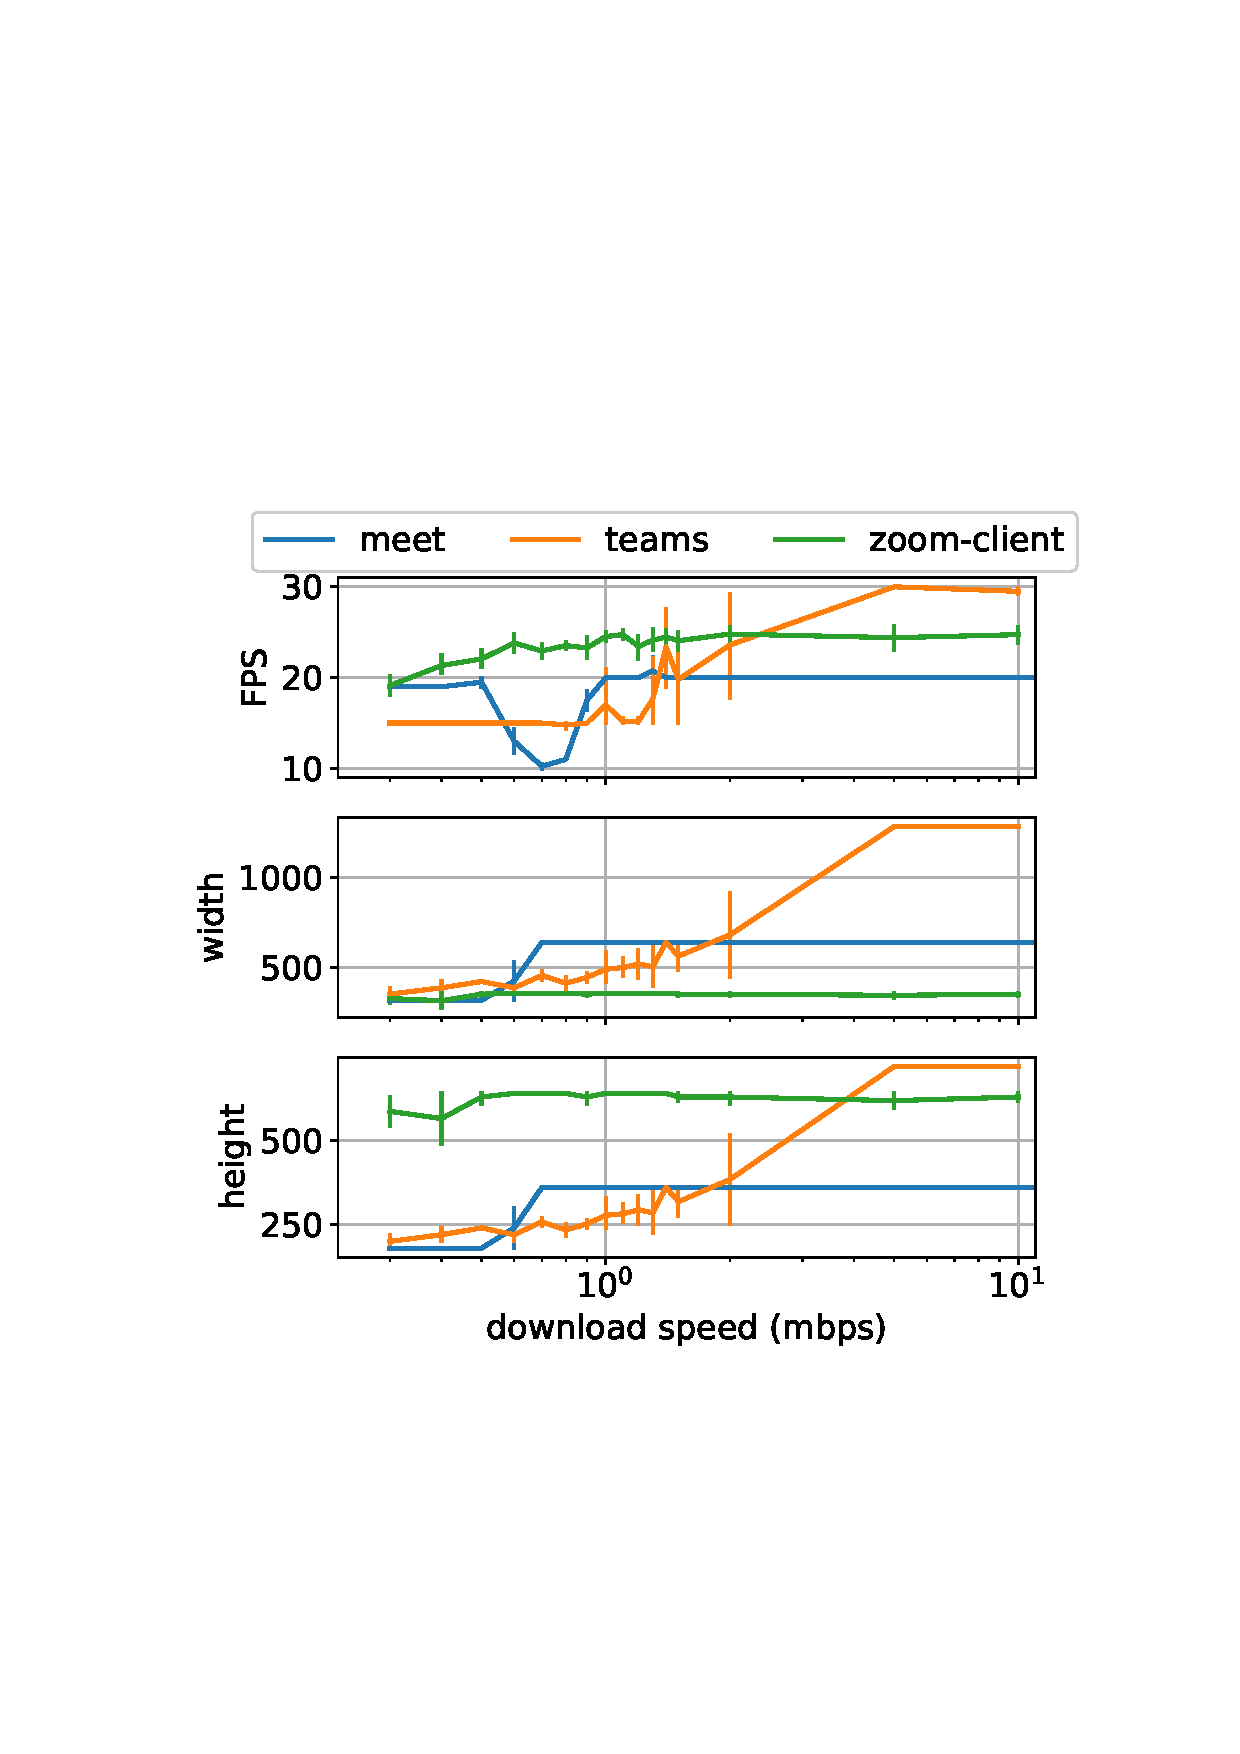
\includegraphics[width=0.35\textwidth,keepaspectratio]{figures/static/downlink_video_qual_meet_teams_zoom.pdf}
    \caption{Downlink bandwidth vs video quality \jamie{I think that width and height are almost always exactly redundant information.  I would choose one.  We should also keep the same colors across plots -- blue shouldn't be both Meet and Zoom client, for instance.}}
    \label{fig:downlink_video_qual}
\end{figure}


\begin{figure}[t]
    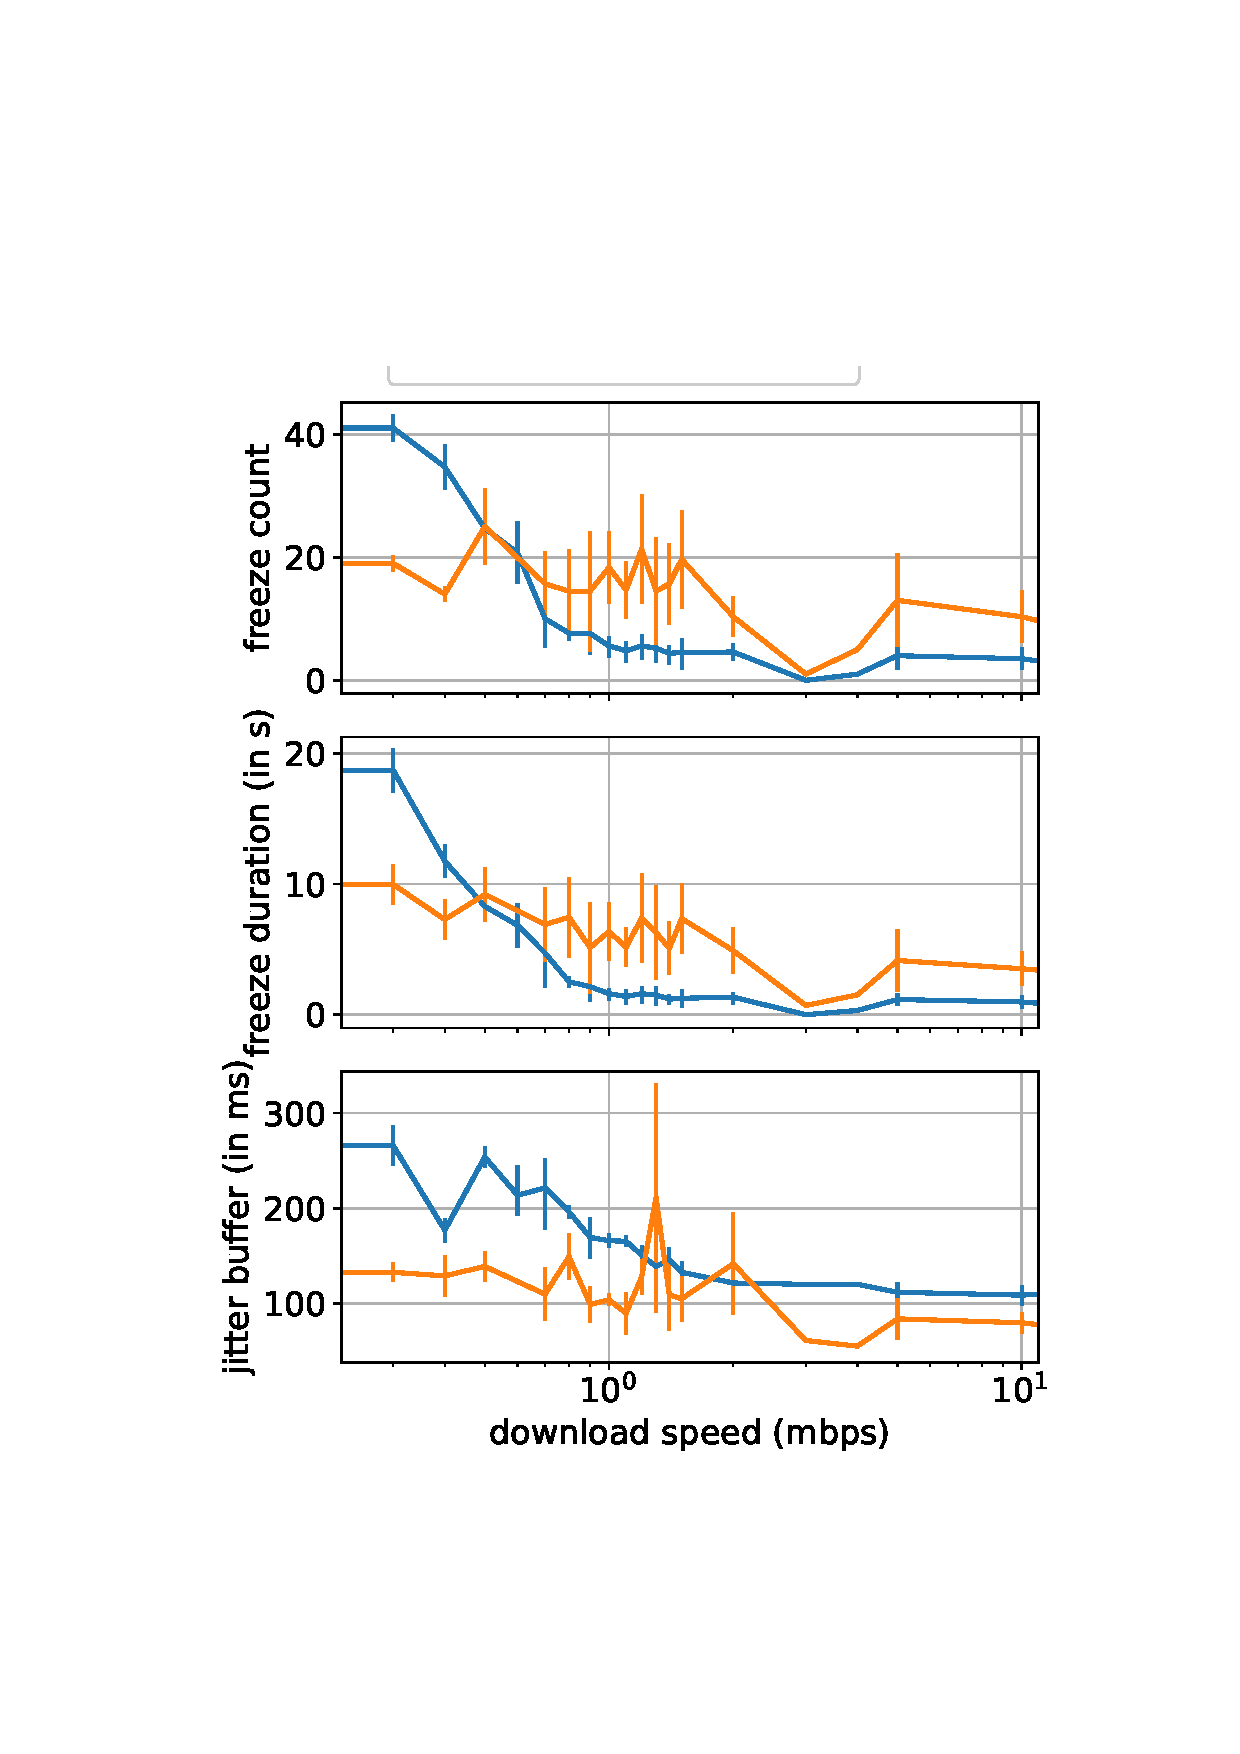
\includegraphics[width=0.35\textwidth,keepaspectratio]{figures/static/downlink_freeze_meet_teams.pdf}
    \caption{Downlink bandwidth and video freezes}
    \label{fig:downlink_freeze}
\end{figure}



\begin{figure}[t]
    \includegraphics[width=0.35\textwidth,keepaspectratio]{figures/static/downlink_qos_zoom.pdf}
    \caption{Downlink bandwidth vs Zoom QoS. \jamie{It looks fishy, that zoom client latency and jitter are identical.  All data from browser seems to be zeroed out?}} 
    \label{fig:downlink_qos_zoom}
\end{figure}
\end{comment}